\documentclass{article}

\usepackage{siunitx} % Provides the \SI{}{} and \si{} command for typesetting SI units
\usepackage{graphicx} % Required for the inclusion of images
\usepackage{epstopdf}
\usepackage{natbib} % Required to change bibliography style to APA
\usepackage{amsmath} % Required for some math elements 
\usepackage{amsmath}
\usepackage{verbatim}
\usepackage{hyperref}

\setlength\parindent{0pt} % Removes all indentation from paragraphs

\renewcommand{\labelenumi}{\alph{enumi}.} 

\renewcommand{\c}[1]{\cos(\theta_{#1})}
\newcommand{\s}[1]{\sin(\theta_{#1})}
\newcommand{\T}[2]{{}^{#1}T_{#2}}
\renewcommand{\O}[2]{{}^{#1}O_{#2}}

\title{Robots Fundamentals:\\
Assignment report} % Title

\author{Rodrigo \textsc{Moreno Carrillo}} % Author name

\date{\today} % Date for the report 
\begin{document}
%call:

\maketitle % Insert the title, author and date

\section{Part 1}
\subsection{Forward kinematics} 

According with the diagram of the Lynxmotion robot depicted in figure \ref{fig:forward.diagram} the correspondig Denavit-Harterverg table using distal convention is:

\begin{table}[h!]
\centering
\begin{tabular}{ c | c c c c}
 n & $a_n$ 	& $\alpha_n$		& $d_n$	& $\theta_n$\\ \hline
 1 & 0 			& 90º				& $d_1$	& $\theta_1$\\  
 2 & $a_2$ 	& 0					& 0			& $\theta_2$\\  
 3 & $a_3$ 	& 0					& 0			& $\theta_3$\\  
 4 & 0 			& 90º				& 0			& $\theta_4$\\  
 5 & 0 			& 0					& $d_5$	& $\theta_5$\\ 
\end{tabular}
\caption{Denavit-Hartenverg table using distal convention}
\label{tab:forward.dh}
\end{table}

In the diagram it is shown that the robot contains five different frames of reference which are described using the parameters in table \ref{tab:forward.dh}. Using these four parameters the frames can be described by the following equations:

\begin{equation}
\label{eq:forward.t_01}
\T{0}{1} = \left[
\begin{array}{cccc}
	\c{1} & 0 & \s{1} & 0 \\
	\s{1} & 0 & -\c{1} & 0 \\
	0 & 1 & 0 & d_1 \\
	0 & 0 & 0 & 1 \\
\end{array}
\right]
\end{equation}

\begin{equation}
\label{eq:forward.t_12}
\T{1}{2} =\left[
\begin{array}{cccc}
	\c{2} & -\s{2} & 0 & a_2\c{2} \\
	\s{2} & \c{2} & 0 & a_2\s{2}  \\
	0 & 0 & 1 & 0 \\
	0 & 0 & 0 & 1 \\
\end{array}
\right]
\end{equation}

\begin{equation}
\label{eq:forward.t_23}
\T{2}{3} =\left[
\begin{array}{cccc}
	\c{3} & -\s{3} & 0 & a_3\c{3} \\
	\s{3} & \c{3} & 0 & a_3\s{3}  \\
	0 & 0 & 1 & 0 \\
	0 & 0 & 0 & 1 \\
\end{array}
\right]
\end{equation}

\begin{equation}
\label{eq:forward.t_34}
\T{3}{4} = \left[
\begin{array}{cccc}
	\c{4} & 0 & \s{4} & 0 \\
	\s{4} & 0 & -\c{4} & 0 \\
	0 & 1 & 0 & 0 \\
	0 & 0 & 0 & 1 \\
\end{array}
\right]
\end{equation}

\begin{equation}
\label{eq:forward.t_45}
\T{4}{5} =\left[
\begin{array}{cccc}
	\c{5} & -\s{5} & 0 & 0 \\
	\s{5} & \c{5} & 0 & 0  \\
	0 & 0 & 1 & d_5\\
	0 & 0 & 0 & 1 \\
\end{array}
\right]
\end{equation}

where

\begin{align*}
a_2 = 9.5 [cm] \\
a_3 = 11 [cm] \\
d_1 = 6.5 [cm] \\
d_5 = 3.2 [cm]
\end{align*}

\begin{figure}
\begin{center}
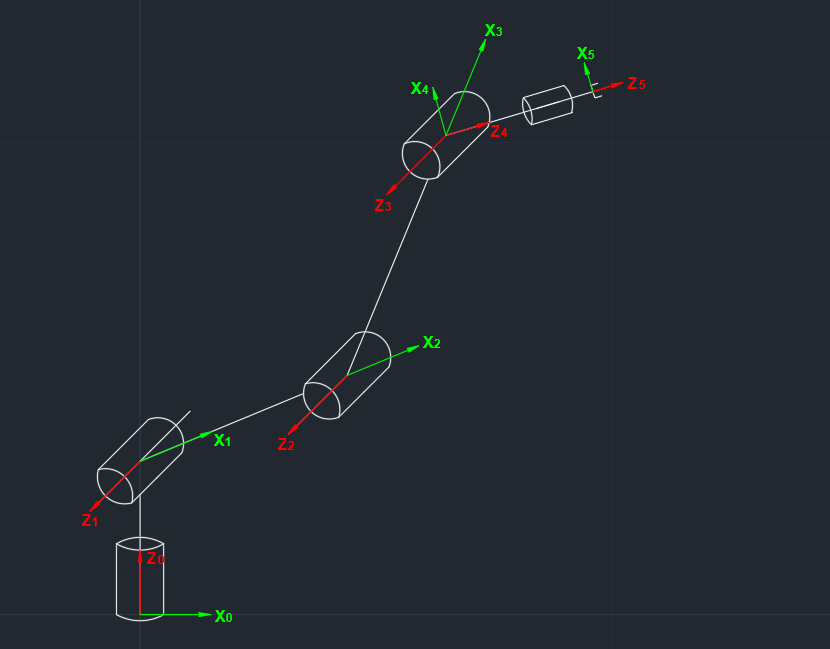
\includegraphics[width=0.8\textwidth]{images/diagram}
\caption{Lynxmotion robot diagram}
\label{fig:forward.diagram}
\end{center}
\end{figure}

Every matrix represents the orientation and displacement of every frame with respect to the previous reference frame. In order to derive the forward kinematics of the robots it is necessary to know the orientation and position of the end effector, the frame at the point $O_5$, with respect to the main reference frame which is the frame with origin at point $O_0$.

In order to know the position and orientation of the end effector after several rotations has been performed, due to the movement of the joints, it is necessary to use the relationship

\begin{equation}
\T{0}{5} = \T{0}{1} \T{1}{2}\T{2}{3}\T{3}{4}\T{4}{5}
\end{equation}

After performing the matrix product, the resultant matrix will be the homogeneous matrix that represents the orientation and position of the frame attached at the end effector, and it will have the following form:

\begin{subequations}
\begin{align}
\T{0}{5} & = \left[
\begin{array}{cccc}
	r_{11} & r_{12} & r_{13} & {}^0Ox_5 \\
	r_{21} & r_{22} & r_{23} & {}^0Oy_5 \\
	r_{31} & r_{32} & r_{33} & {}^0Oz_5 \\
	0 & 0 & 0 & 1 \\
\end{array}
\right] \\
& = \left[
\begin{array}{cc}
	R & {}^0O_5 \\
	 0 & 1 \\
\end{array}
\right] 
\end{align}
\end{subequations}

where $R$ is the rotation matrix of the fifth frame with respect to main frame and ${}^0O_5$ is the coordinate vector of point $O_5$ with respect to main frame. This point is also the desired point of the end effector. This matrix is a function of the variables $\theta_1 ... \theta_5$.

\begin{equation*}
{}^0O_5 = \left[
\begin{array}{c}
	{}^0Ox_5 \\
	{}^0Oy_5 \\
	{}^0Oz_5 \\
\end{array}
\right] = \left[
\begin{array}{c}
	{}^0P_x \\
	{}^0P_y \\
	{}^0P_z \\
\end{array}
\right] = {}^0P
\end{equation*}

To perform the computing of the forward kinematics of the Lynxmotion it was created a function in Matlab that receives as input the vector $Q=[\theta_1 \theta_2 \theta_3 \theta_4 \theta_5]^T$ and it gives the position ${}^0P$ and orientation $R$ of the end effector as output. The code of the function can be found in appendix \ref{apendix:LynxFK}.

\subsection{Workspace}
To have a representation of the workspace, it was necessary to measure the physical operational range of every joint in order to establish the domain of every variable $\theta_i$, the results are in table \ref{tab:workspace.range}.

\begin{table}[h!]
\centering
\begin{tabular}{ c | c }
Variable		& Operational range [º]\\ \hline
$\theta_1$	& [-90, 90]\\
$\theta_2$	& [0, 135]\\
$\theta_3$	& [-135, 30]\\
$\theta_4$	& [0, 180]\\
$\theta_5$	& [-90, 90]
\end{tabular}
\caption{Operational range of joint variables}
\label{tab:workspace.range}
\end{table}

Once the range of the variables has been determined, it can be simulated the movement of every joint in its corresponding operational range to create a representation of the reachable 3D space. The space generated by all the points that can be reached by the end effector of the robot is called workspace. The used code to perform the simulation can be found in appendix \ref{apendix:workspace}.

\begin{figure}
\begin{center}
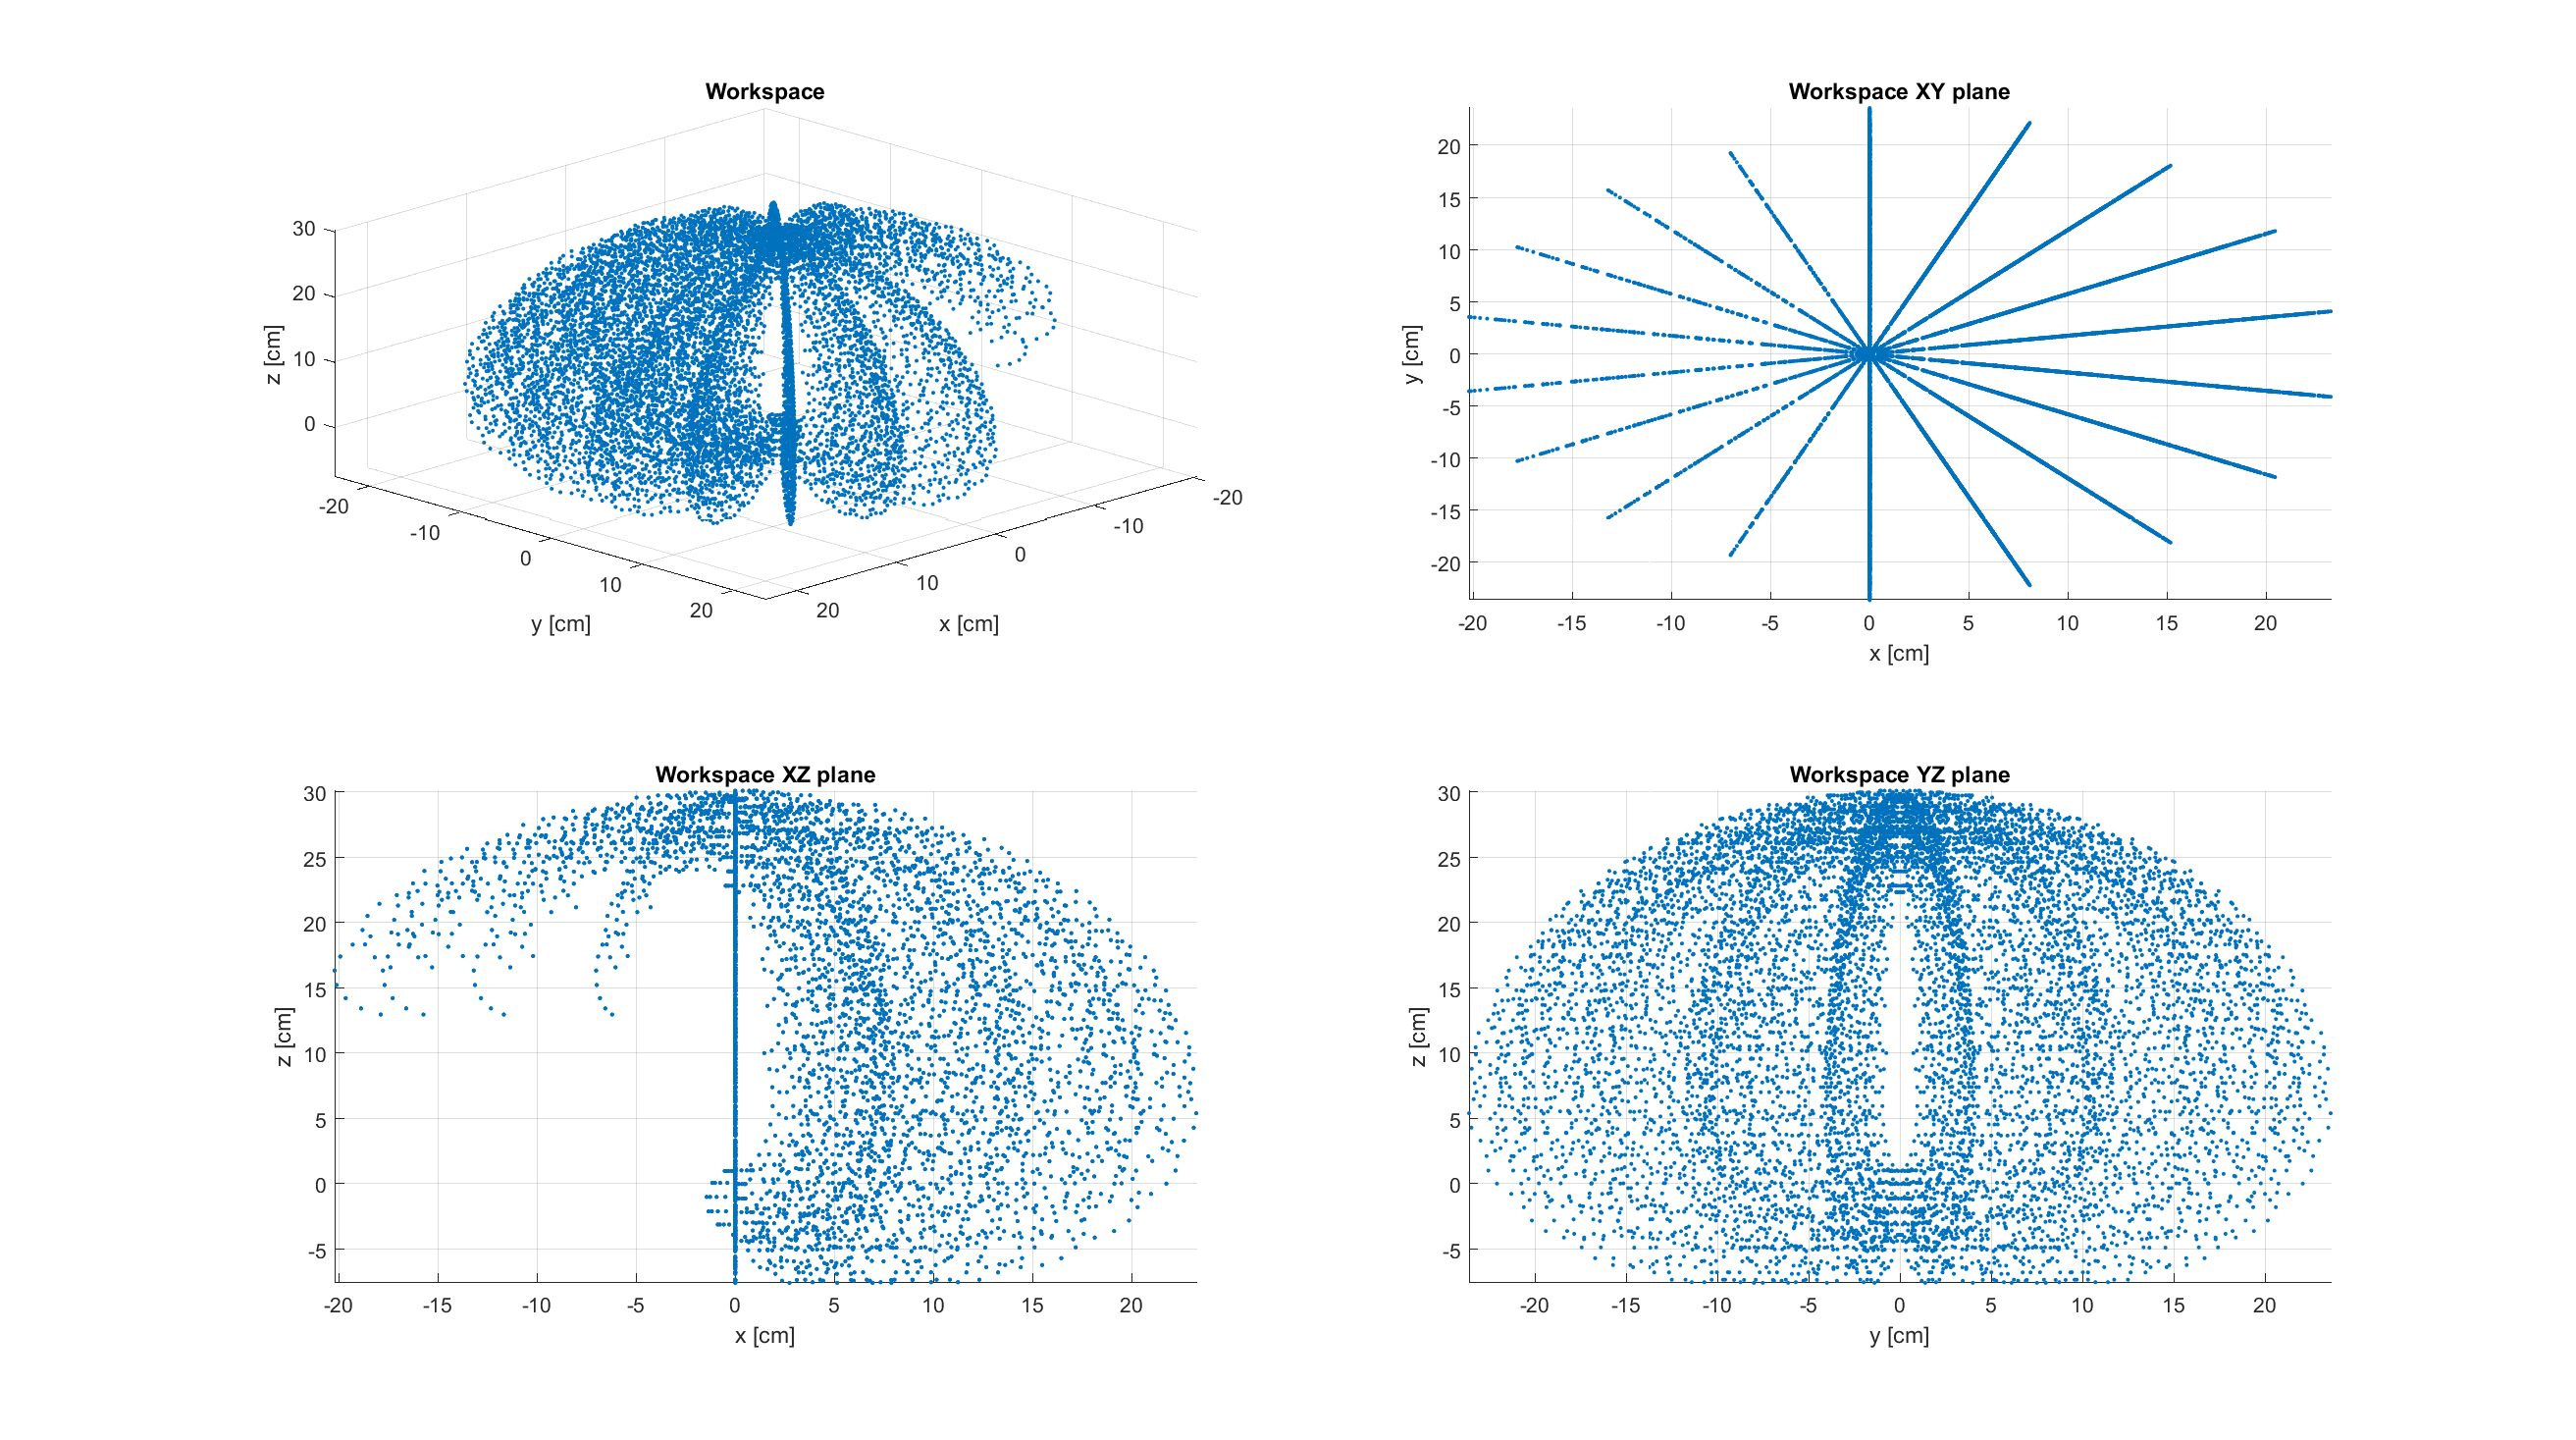
\includegraphics[width=\textwidth]{images/Workspace}
\caption{Lynxmotion robot workspace}
\label{fig:workpace.workspace}
\end{center}
\end{figure}

The workspace of the Lynxmotion robot is depicted in figure \ref{fig:workpace.workspace}, the picture shows a 3D view of the space, while the other three view shows the planes YX, ZX and ZY respectively.

\subsection{Inverse kinematics}
The concept of inverse kinematics is finding joint valuables given the specific position and orientation of the end effector. Concretely, there are five joints valuables need to be worked out, namely  $\theta_1$,  $\theta_2$,  $\theta_3$,  $\theta_4$,  $\theta_5$.

\subsubsection{Finding  $\theta_1$}
Since the x and y position of the end effector are only decided by the rotation of joint 1, we can project the manipulator into the horizontal plane of the frame 0. Therefore, we can derive the expression of  $\theta_1$ as

\begin{equation}
\theta_1 = atan2(Py, Px)
\end{equation}

\subsubsection{Finding  $\theta_2$, $\theta_3$}
In order to simplify the configuration, we can extract link 2 and link 3 from the whole manipulator, hence the link 2 and link 3 would be a planar mechanism. The next step is to find the origin coordinates of frame 3 with respect to frame 1, namely $\O{1}{3}$, which can be derived from the matrix of $\T{1}{3}$. Furthermore, $\T{1}{3}$ can be expressed as the product

\begin{align}
\label{eq:inverse.t_13}
\T{0}{1}\T{1}{3} & = \T{0}{3} \nonumber \\
{(\T{0}{1})}^{-1}\T{0}{1}\T{1}{3}& = {(\T{0}{1})}^{-1} \T{0}{3} \nonumber \\
\T{1}{3} & = \T{1}{0} \T{0}{3}
\end{align}

According to the equation (\ref{eq:inverse.t_13}), we need to get the matrixes $\T{1}{0}$ and $\T{0}{3}$ respectively. $\T{1}{0}$ is easy to get from the inverse matrix of $\T{0}{1}$, which should be 

\begin{equation}
\label{eq:inverse.t_10}
{(\T{0}{1})}^{-1} = \T{1}{0} = \left[
\begin{array}{cccc}
	\c{1} & \s{1} & 0 & 0 \\
	0 & 0 & 1 & -d_1 \\
	\s{1} & -\c{1} & 0 & 0 \\
	0 & 0 & 0 & 1 \\
\end{array}
\right]
\end{equation}

As for  $\T{0}{3}$, we only focus on the displacement part $\O{0}{3}$(the last column of $\T{0}{3}$).

\begin{equation}
\label{eq:inverse.t_03}
\T{0}{3} = \left[ \begin{array}{cccc}
	\cdot & \cdot & \cdot & {}^0O_{3x} \\
	\cdot & \cdot & \cdot & {}^0O_{3y} \\
	\cdot & \cdot & \cdot & {}^0O_{3z} \\
	0 & 0 & 0 & 1 \\
\end{array} \right]
\end{equation}

Furthermore, $Z_5$ is aligned with link 4 whose length is $d_5$, so $\O{0}{3}$ can be calculated by

\begin{equation}
\label{eq:inverse.O_03}
\begin{aligned}
\O{0}{3} & = {}^0P - d_5 R\left[
\begin{array}{c}
	0 \\
	0 \\
	1 \\
\end{array} \right]  \\
\left[
\begin{array}{c}
	{}^0O_{3x} \\
	{}^0O_{3y} \\
	{}^0O_{3z} \\
\end{array} \right] & = \left[
\begin{array}{c}
	{}^0P_x \\
	{}^0P_y \\
	{}^0P_z \\
\end{array}
\right] - d_5 \left[ \begin{array}{c}
	{}r_{13} \\
	{}r_{23} \\
	{}r_{33} \\
\end{array} \right]
\end{aligned}
\end{equation}

Then, $\T{1}{3}$ can be computed by substituting (\ref{eq:inverse.t_10}), (\ref{eq:inverse.t_03}) and (\ref{eq:inverse.O_03}) in (\ref{eq:inverse.t_13}). Lastly, as only the fourth column is needed at this moment, equation (\ref{eq:inverse.t_13_expanded}) only shows the last column for simplicity.

\begin{equation}
\label{eq:inverse.t_13_expanded}
\T{1}{3} = \left[ \begin{array}{cccc}
	\cdot & \cdot & \cdot & \O{0}{3x} \c{1} + \O{0}{3y} \s{1} \\
	\cdot & \cdot & \cdot & \O{0}{3z}-d_1 \\
	\cdot & \cdot & \cdot & \O{0}{3x} \s{1}-\O{0}{3y} \c{1} \\
	0 & 0 & 0 & 1 \\
\end{array} \right]
\end{equation}

Therefore, we found the coordinates of frame 3 with respect to frame 1(namely $\O{1}{3}$), as denoted in equation (\ref{eq:inverse.O_13}). Then the solutions of  $\theta_2$ and  $\theta_3$ can be worked out by the geometrical method mentioned in the lecture. There are 2 solutions as a result of redundancy, which is shown below in figure \ref{fig:theta_2,theta_3}.

\begin{align}
\label{eq:inverse.O_13}
\O{1}{3} = 
\left[ \begin{array}{c}
	\O{1}{3x} \\
	\O{1}{3y} \\
	\O{1}{3z} \\
\end{array} \right] = \left[ \begin{array}{c}
	\O{0}{3x} \c{1} + \O{0}{3y} \s{1} \\
	\O{0}{3z}-d_1 \\
	\O{0}{3x} \s{1}-\O{0}{3y} \c{1} \\
\end{array} \right]
\end{align}

\begin{figure}
\begin{center}
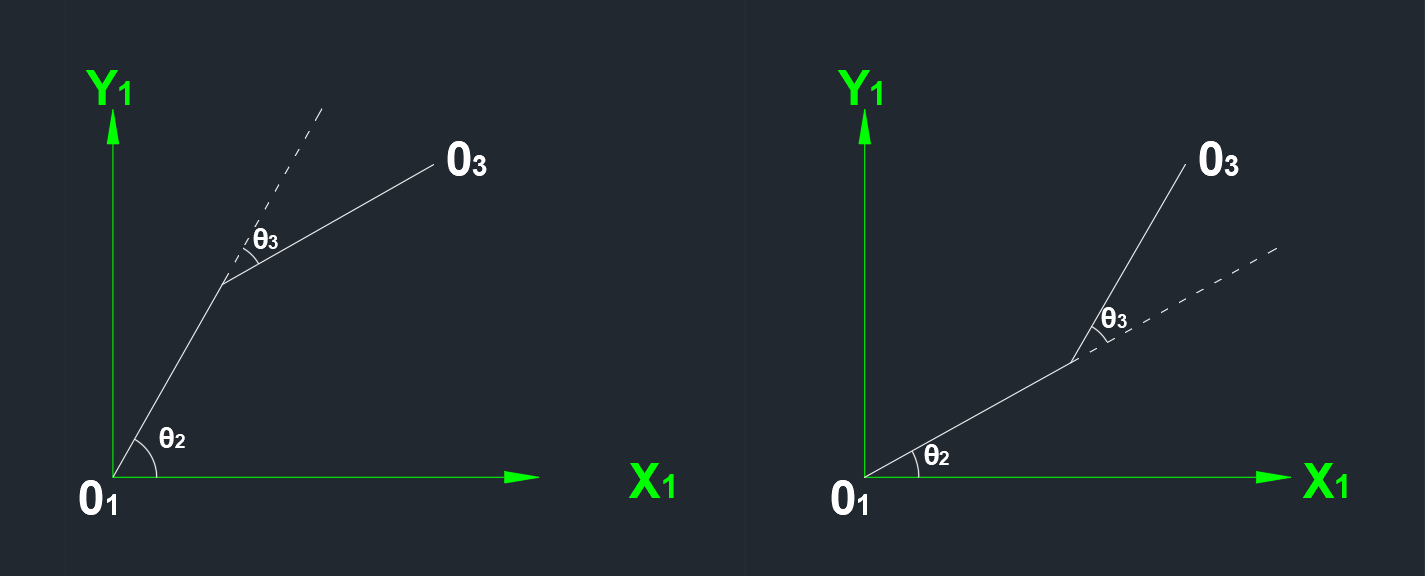
\includegraphics[width=\textwidth]{images/theta2,theta3}
\caption{Graphical representation of the two solutions for $\theta_2$ and $\theta_3$, namely elbow left and elbow right}
\label{fig:theta_2,theta_3}
\end{center}
\end{figure}

Applying the law of cosines and using the coordinates of point $O_3$ with respect to $O_1$, we can derive the expression of $\theta_3$ that
\begin{equation*}
\c{3} = \frac{\O{1}{3x}^2 + \O{1}{3y}^2 - a_2^2 - a_3^2}{2a_2a_3}\qquad
\end{equation*}
while sine will have two possible values, a positive and a negative value, which will lead to the two solutions depicted above.
\begin{equation*}
\s{3} = \pm\sqrt{1-\c{3}^2}
\end{equation*}

\begin{equation*}
\theta_{3} = \begin{cases} 
   \theta_{3_1} & \text{for } {\s{3}}^+ \\
   \theta_{3_2} & \text{for } {\s{3}}^-
  \end{cases}
\end{equation*}

\begin{equation}
\theta_{3} = atan2(\s{3},\c{3})
\end{equation}

Finally, $\theta_2$ can be computed from the angle of $\O{1}{3}$ once that $\theta_3$ is known.

\begin{equation}
\theta_{2} = atan2(\O{1}{3y},\O{1}{3x})-atan2(\sin(b),\cos(b) )
\end{equation}
where
\begin{equation*}
\sin(b)= \frac{a_3\s{3}}{\sqrt{\O{1}{3x}^2+\O{1}{3y}^2}}
\end{equation*}

Accordingly with the dependency of $\theta_2$ on the value of $\theta_3$, this variable will also have two solutions. The set of two solutions for both variables, creates the two possible configurations, elbow right for $\theta_3^+$ and elbow left for $\theta_3^-$, as depicted in figure \ref{fig:theta_2,theta_3}.

\subsubsection{Finding $\theta_4$}
The algebraic was used method to work out $\theta_4$. The core idea is building an equation of $\theta_4$ from the element of transformation matrix $\T{3}{5}$.Now,$\theta_1$, $\theta_2$, $\theta_3$ are already known. Combined with  $\T{0}{5}$,  $\T{3}{5}$ can be derived from

\begin{align}
\label{eq:inverse.t_35}
\T{0}{3}\T{3}{5} & = \T{0}{5} \nonumber \\
{(\T{0}{3})}^{-1}\T{0}{3}\T{3}{5}& = {(\T{0}{3})}^{-1} \T{0}{5} \nonumber \\
\T{3}{5} & = \T{3}{0} \T{0}{5}
\end{align}

where

\begin{equation}
\label{eq:inverse.t_30}
\T{3}{0} = \T{3}{2}\T{2}{1}\T{1}{0} 
\end{equation}

Each element on the right side of equation \ref{eq:inverse.t_35} depends on $\theta_1$, $\theta_2$ and $\theta_3$ which are already known. It is important to remark that there exists two versions of $\T{3}{2}$ and $\T{2}{1}$ as there are two solutions. Therefore, $\T{3}{5}$ will have two versions, both with a form like this:

\begin{equation}
\label{eq:inverse.t_35_expanded}
\T{3}{5}= \left[
\begin{array}{cccc}
	\cdot & \cdot & \cdot & \O{3}{5x} \\
	\cdot & \cdot & \cdot & \O{3}{5y} \\
	\cdot & \cdot & \cdot & \O{3}{5z} \\
    0 & 0 & 0 & 1 \\
\end{array}
\right] 
\end{equation}

On the other hand, another way to get $\T{3}{5}$ with variable $\theta_4$ is as a product of matrix (\ref{eq:forward.t_34}) and matrix (\ref{eq:forward.t_45}), which is

\begin{equation}
\begin{aligned}
\label{eq:inverse.t_35_forward}
\T{3}{5} = \T{3}{4} \T{4}{5} & =
\left[
\begin{array}{cccc}
	\c{4} & 0 & \s{4} & 0 \\
	\s{4} & 0 & -\c{4} & 0 \\
	0 & 1 & 0 & 0 \\
	0 & 0 & 0 & 1 \\
\end{array}
\right] \left[
\begin{array}{cccc}
	\c{5} & -\s{5} & 0 & 0 \\
	\s{5} & \c{5} & 0 & 0  \\
	0 & 0 & 1 & d_5\\
	0 & 0 & 0 & 1 \\
\end{array}
\right] \\
& = \left[
\begin{array}{cccc}
	\cdot & \cdot & \cdot & d_5\s{4} \\
	\cdot & \cdot & \cdot & -d_5\c{4}\\
	\cdot & \cdot & \cdot & 0\\
    0 & 0 & 0 & 1 \\
\end{array}
\right] 
\end{aligned}
\end{equation}

Thus, $\T{3}{5}$ has been derived in two ways, which can be used to create an equation system to solve for $\theta_4$. By equalising the last column of (\ref{eq:inverse.t_35_expanded}) and (\ref{eq:inverse.t_35_forward}) we obtain:

\begin{equation}
\s{4} = \frac{\O{3}{5x}}{d_5}
\qquad
\c{4} = -\frac{\O{3}{5y}}{d_5}
\end{equation}
therefore
\begin{equation}
\theta_{4} = atan2(\s{4},\c{4})
\end{equation}

As a result of the two versions of (\ref{eq:inverse.t_35_expanded}), $\theta_4$ will also have two solutions that must be computed in the same way for both configurations.

\subsubsection{Finding $\theta_5$}
The method of calculating $\theta_5$ is the similar to finding $\theta_4$. we try to get the matrix  $\T{4}{5}$ from two ways. The one with variable $\theta_5$ is obviously expressed in equation \ref{eq:forward.t_45}.

Another means of representing $\T{4}{5}$ is 
\begin{equation}
\label{eq:inverse.t_45}
\T{4}{5} = \T{4}{0} \T{0}{5}
\end{equation}
where
\begin{equation*}
\T{4}{0} = \T{4}{3}\T{3}{0}
\end{equation*}
Therefore, the equation (\ref{eq:inverse.t_45}) depends on the inverse of (\ref{eq:forward.t_34}), (\ref{eq:inverse.t_03}) and $\T{0}{5}$ which is given as the desired position and orientation. 

It seems that $\theta_5$ should also have two solutions since $\s{4}$ and $\c{4}$ have 2 pairs of solutions and the expression of $\T{4}{0}$ contains $\s{4}$ and $\c{4}$. Whereas, it turns out that $\T{4}{0}$ only have one value due to the same computing result of 2 pairs of $\s{4}$ and $\c{4}$.For simplicity, we use (a,b) to represent each element of $\T{4}{5}$(a,b are the numble of rows and columns). Thus, $\s{5}$ and $\c{5}$ can be written as

\begin{equation}
\s{5} = \T{4}{5}(2,1)
\qquad
\c{5} = \T{4}{5}(1,1)
\end{equation}
Hence,the solutions of $\theta_5$ is
\begin{equation}
\theta_{5} = atan2(\s{5},\c{5})
\end{equation}

\subsection{Task plan}
The chosen task was to imagine the problem of taking three objects and stick them to a wall, this might be considered as a pick and place task. In this case the robot should take an object and take it to its final position, then take the second object and place it in the second position and finally perform the same process for the last object.

The points where chosen by inspecting the workspace and placing them in the workspace of the robot. They can be seen in the chart of figure \ref{fig:points.points}.

\begin{figure}
\begin{center}
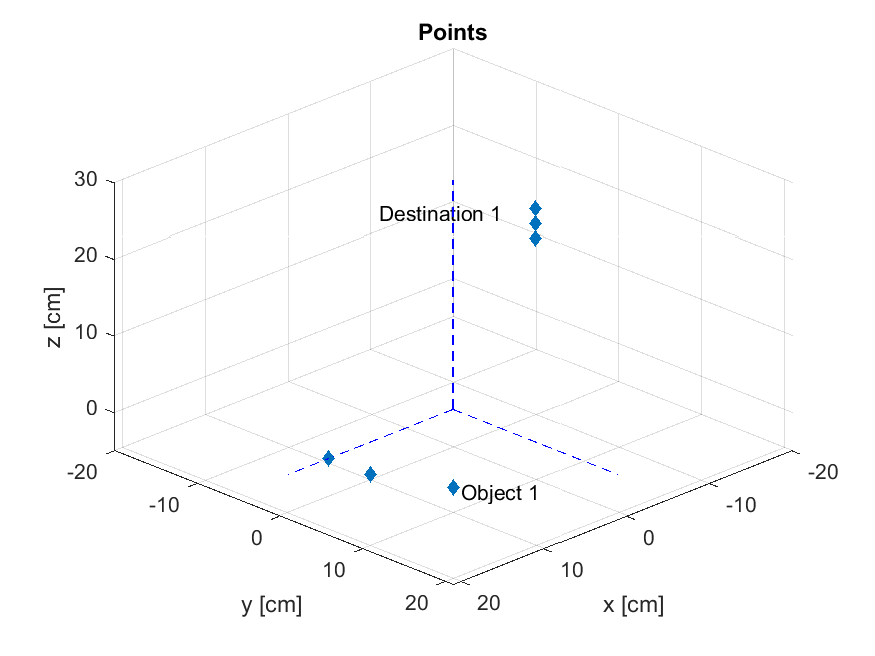
\includegraphics[width=\textwidth]{images/Points}
\caption{Chosen points for the pick and place task}
\label{fig:points.points}
\end{center}
\end{figure}

\subsection{Forward kinematics test}
In order to test the forward kinematics po

\subsection{Inverse kinematics test and animation}

\subsection{Trajectories}

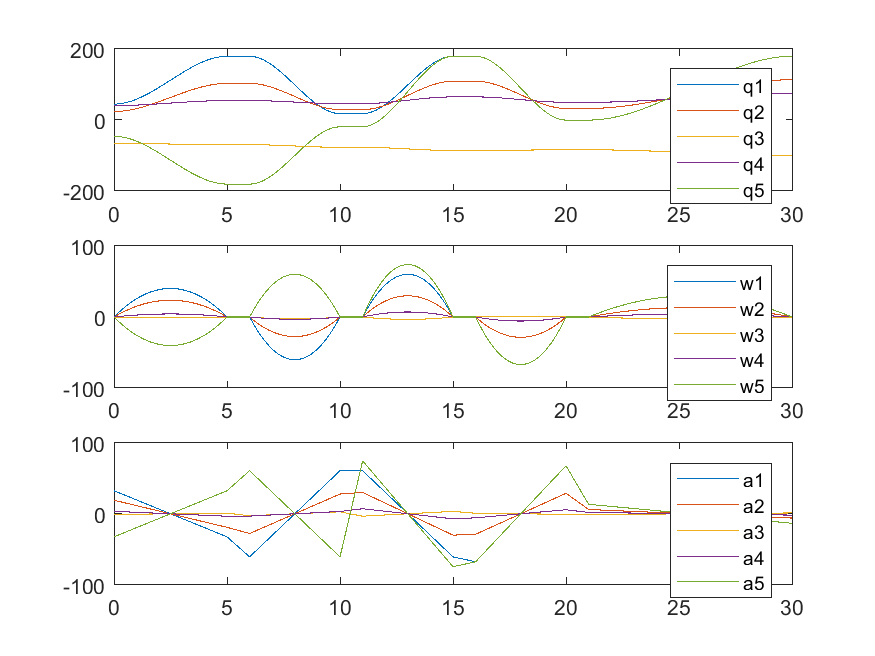
\includegraphics[scale=1]{images/JointTrayectories}

\section{Part 2}


\subsection{This is a subsection} %What do you think about it? Should others read it?

\appendix
\section{Matlab codes}
\subsection{Forward kinematics (LynxFK function)}
\label{apendix:LynxFK}
\verbatiminput{code/Part1/LynxFK.m}

\subsection{Workspace (workspace script)}
\label{apendix:workspace}
\verbatiminput{code/Part1/workspace_script.m}


%----------------------------------------------------------------------------------------
%	BIBLIOGRAPHY
%----------------------------------------------------------------------------------------

\bibliographystyle{plain}
%\bibliography{sample}

\end{document}
